
%
%  $Description: Author guidelines and sample document in LaTeX 2.09$ 
%
%  $Author: ienne $
%  $Date: 1995/09/15 15:20:59 $
%  $Revision: 1.4 $
%

\documentclass[times, 10pt,twocolumn]{article} 
\usepackage{latex8}
\usepackage{times}
\usepackage{graphicx}
\usepackage{subcaption}
\usepackage{algorithm}
\usepackage{algorithmic}
\usepackage{adjustbox}
\usepackage{enumitem}
\usepackage{enumitem}


%\documentstyle[times,art10,twocolumn,latex8]{article}

%------------------------------------------------------------------------- 
% take the % away on next line to produce the final camera-ready version 
\pagestyle{empty}

%------------------------------------------------------------------------- 
\begin{document}

% \title{Epidemics Graph Neural Network Node Classification}
\title{Epidemics Graph Neural Network Link Prediction}

\author{Jaykumar Patel\\
patel.jay4802@utexas.edu\\
% For a paper whose authors are all at the same institution, 
% omit the following lines up until the closing ``}''.
% Additional authors and addresses can be added with ``\and'', 
% just like the second author.
\and
Afnan Mir\\
afnanmir@utexas.edu\\
}

\maketitle
\thispagestyle{empty}

\begin{abstract}
The COVID-19 pandemic showed that contact tracing helped mitigate the spread of the virus. However, manual contact tracing is slow and prone to inaccuracies. Thus, this project aims to automate contact tracing by utilizing Graph Neural Networks (GNNs) for link prediction. Our network analysis shows that the contact network is mostly exponential with hints of scale-free properties. Additionally, our analysis identifies a discernible pattern in mobility, characterized by an increase in travel during the weekends. Furthermore, we were able to achieve an AUC of 0.91 for static link prediction by using the GCN architecture and performing feature engineering. We then performed a temporal link prediction, which uses previous contact networks to predict future contacts. We achieved an ROC AUC score of 0.79 on nodes that were seen during training, and 0.54 on nodes that were not seen during training.
\end{abstract}


%------------------------------------------------------------------------- 
\Section{Introduction and Motivation}

When COVID-19 first appeared, manual contact tracing was deployed to mitigate the initial outbreak. Contact tracing is the process of tracking how the virus spreads by identifying people who may have come in contact with an infected person, and then asking them to isolate and get tested.

However, the pandemic revealed that the COVID-19 virus spread faster than manual contact tracing \cite{flaxman2020estimating}. Thus, this project's objective is to automate contact tracing by incorporating machine learning using GNNs to hopefully increase the mitigation of the spread of COVID-19 when compared to manual contact tracing. Firstly, we will create and analyze contact networks. Then we will use GNNs to perform static link prediction using a 5-Day Contact Network. Finally, we will perform temporal link prediction on the daily contact networks.

% - What is the big picture? What is the main objective of this project?
% - Why is this project interesting?

%------------------------------------------------------------------------- 

\Section{Previous Work}
% Methods for predicting the spread of COVID-19 include mathematical models, traditional ML models, and graph-based ML models. 

% One example of a mathematical model is the SEIRD model, which attempts to predict the change in Susceptible, Exposed, Infected, Recovered, and Deceased people over time through use of differential equations. This model is used to simulate the spread of the virus over time \cite{SEIRD-LSTM}.
% % (https://www.frontiersin.org/articles/10.3389/fpubh.2021.727274/full)
% SIR is simpler version of the SIERD model that attempts to perform the same task \cite{SIR}.
% % https://www.medrxiv.org/content/10.1101/2020.05.15.20103077v2

% Traditional ML models have also been used to predict the spread of COVID-19. For example, Long Short-Term Memory (LSTM) models have been used to predict the number of cases over time \cite{SEIRD-LSTM}. 
% % https://www.frontiersin.org/articles/10.3389/fpubh.2021.727274/full
% Another approach utilizes a hybrid of SIRD and LSTM to account for time dependent parameters of the SIRD model \cite{SIRD-LSTM-hybrid}.
% % https://www.nature.com/articles/s41598-022-06992-0

% Furthermore, graph-based ML models, such as GNNs, have been used on mobility data to predict the number of cases and hospitalizations \cite{positivity-hospitalization-GNN}.
% % https://www.ncbi.nlm.nih.gov/pmc/articles/PMC10066232/#:~:text=Message%20passing%20instances%20of%20GNNs,as%20well%20as%20hospitalization%20rates.
% GNNs can also be used for link prediction, which is useful for contact tracing \cite{contact-tracing-GNN}. 
% % https://proceedings.neurips.cc/paper_files/paper/2018/file/53f0d7c537d99b3824f0f99d62ea2428-Paper.pdf

% Methods for predicting the spread of COVID-19 include mathematical models, traditional ML models, and graph-based ML models. 

Mathematical models, classical machine learning models, and graph-based machine learning models have been used to predict virus spread. 

The SEIRD model is a mathematical model that predicts the change in Susceptible, Exposed, Infected, Recovered, and Deceased people over time by using differential equations. \cite{SEIRD-LSTM}. The Susceptible-Infected-Recovered (SIR) model is a simpler version of the SEIRD model \cite{SIR}.

The Long Short Term Memory model is a machine learning model that has been used to predict the number of cases over time \cite{SEIRD-LSTM}. A hybrid of SIRD and LSTM helps account for time-dependent parameters of the SIRD model \cite{SIRD-LSTM-hybrid}. Also, GNNs, which are graph-based ML models, have been used on mobility data to predict virus spread and for link prediction for contact tracing \cite{positivity-hospitalization-GNN}\cite{contact-tracing-GNN}.

Additionally, there have been studies done on performing graph learning on networks that are dynamic in nature, such as contact networks. The Temporal Graph Network (TGN) framework allows us to perform deep learning tasks on a sequence of graphs by using memory modules and graph-based operators \cite{rossi2020temporal}

We hope to build off of these previous works by utilizing GNNs and other deep learning techniques to be able to predict contacts between individuals. This is a non-trivial and novel task, as it requires the model to potentially learn a graph's structure based on its structure at previous time steps as well as node features.


\Section{Approach}
\subsection{Network Generation and Simulation}
% We used the foursquare dataset to build a contact graph of Austin, Texas \cite{DVN/PFLAH4_2020}. Each entry contains data such as a device ID, a location ID, UTC date and hour, and a dwell time, which all tell us when a person visited a location and for how much time. Given this data, we generated a contact graph for people in Austin.

We used the Foursquare dataset from the months of July and August 2020 to build contact networks of Austin, TX \cite{DVN/PFLAH4_2020}. Each entry contains a device ID, a location ID, a UTC date and hour, and a dwell time, which tell us when and how long a person visited a location. Given this data, we generated a contact graph of Austin.

% We used data only from July 1st, 2020 to generate a sample network. Our nodes were all the unique device IDs in the dataset, which correspond to people. For our edges, we used the following logic: we ignored entries with a dwell time less than 60 minutes, as we assumed this not enough time to make significant contact with others. Then, we used the UTC date and hour with the dwell time to determine the arrival and departure time interval for each entry. We then compared every entry with every other entry. If the entries' locations were the same and if intervals overlapped by at least 60 minutes, we considered this as a contact between the two people and added an edge between them. Figure \ref{fig:toy_label} shows an example of a sample contact network generation. 

Firstly, we used data from July 1st, 2020 to July 5th, 2020 to create a sample contact network. Our nodes were all the unique device IDs in the dataset, which correspond to people. For our edges, we used the following logic: we ignored entries with a dwell time of less than 60 minutes, as we assumed this was not enough time to make significant contact with others. Then, we used the UTC date and hour with the dwell time to determine the arrival and departure time interval for each entry. We then compared every entry with every other entry. If the entries' locations were the same and if intervals overlapped by at least 60 minutes, we considered this as a contact between the two people and added an edge between them. We will call this the 5-Day Contact Network. This network captures the meaningful contacts that occurred between people from July 1st, 2020 to July 5th, 2020. Figure \ref{fig:toy_label} shows an example of a sample contact network generation. 

\begin{figure}
    \centering
    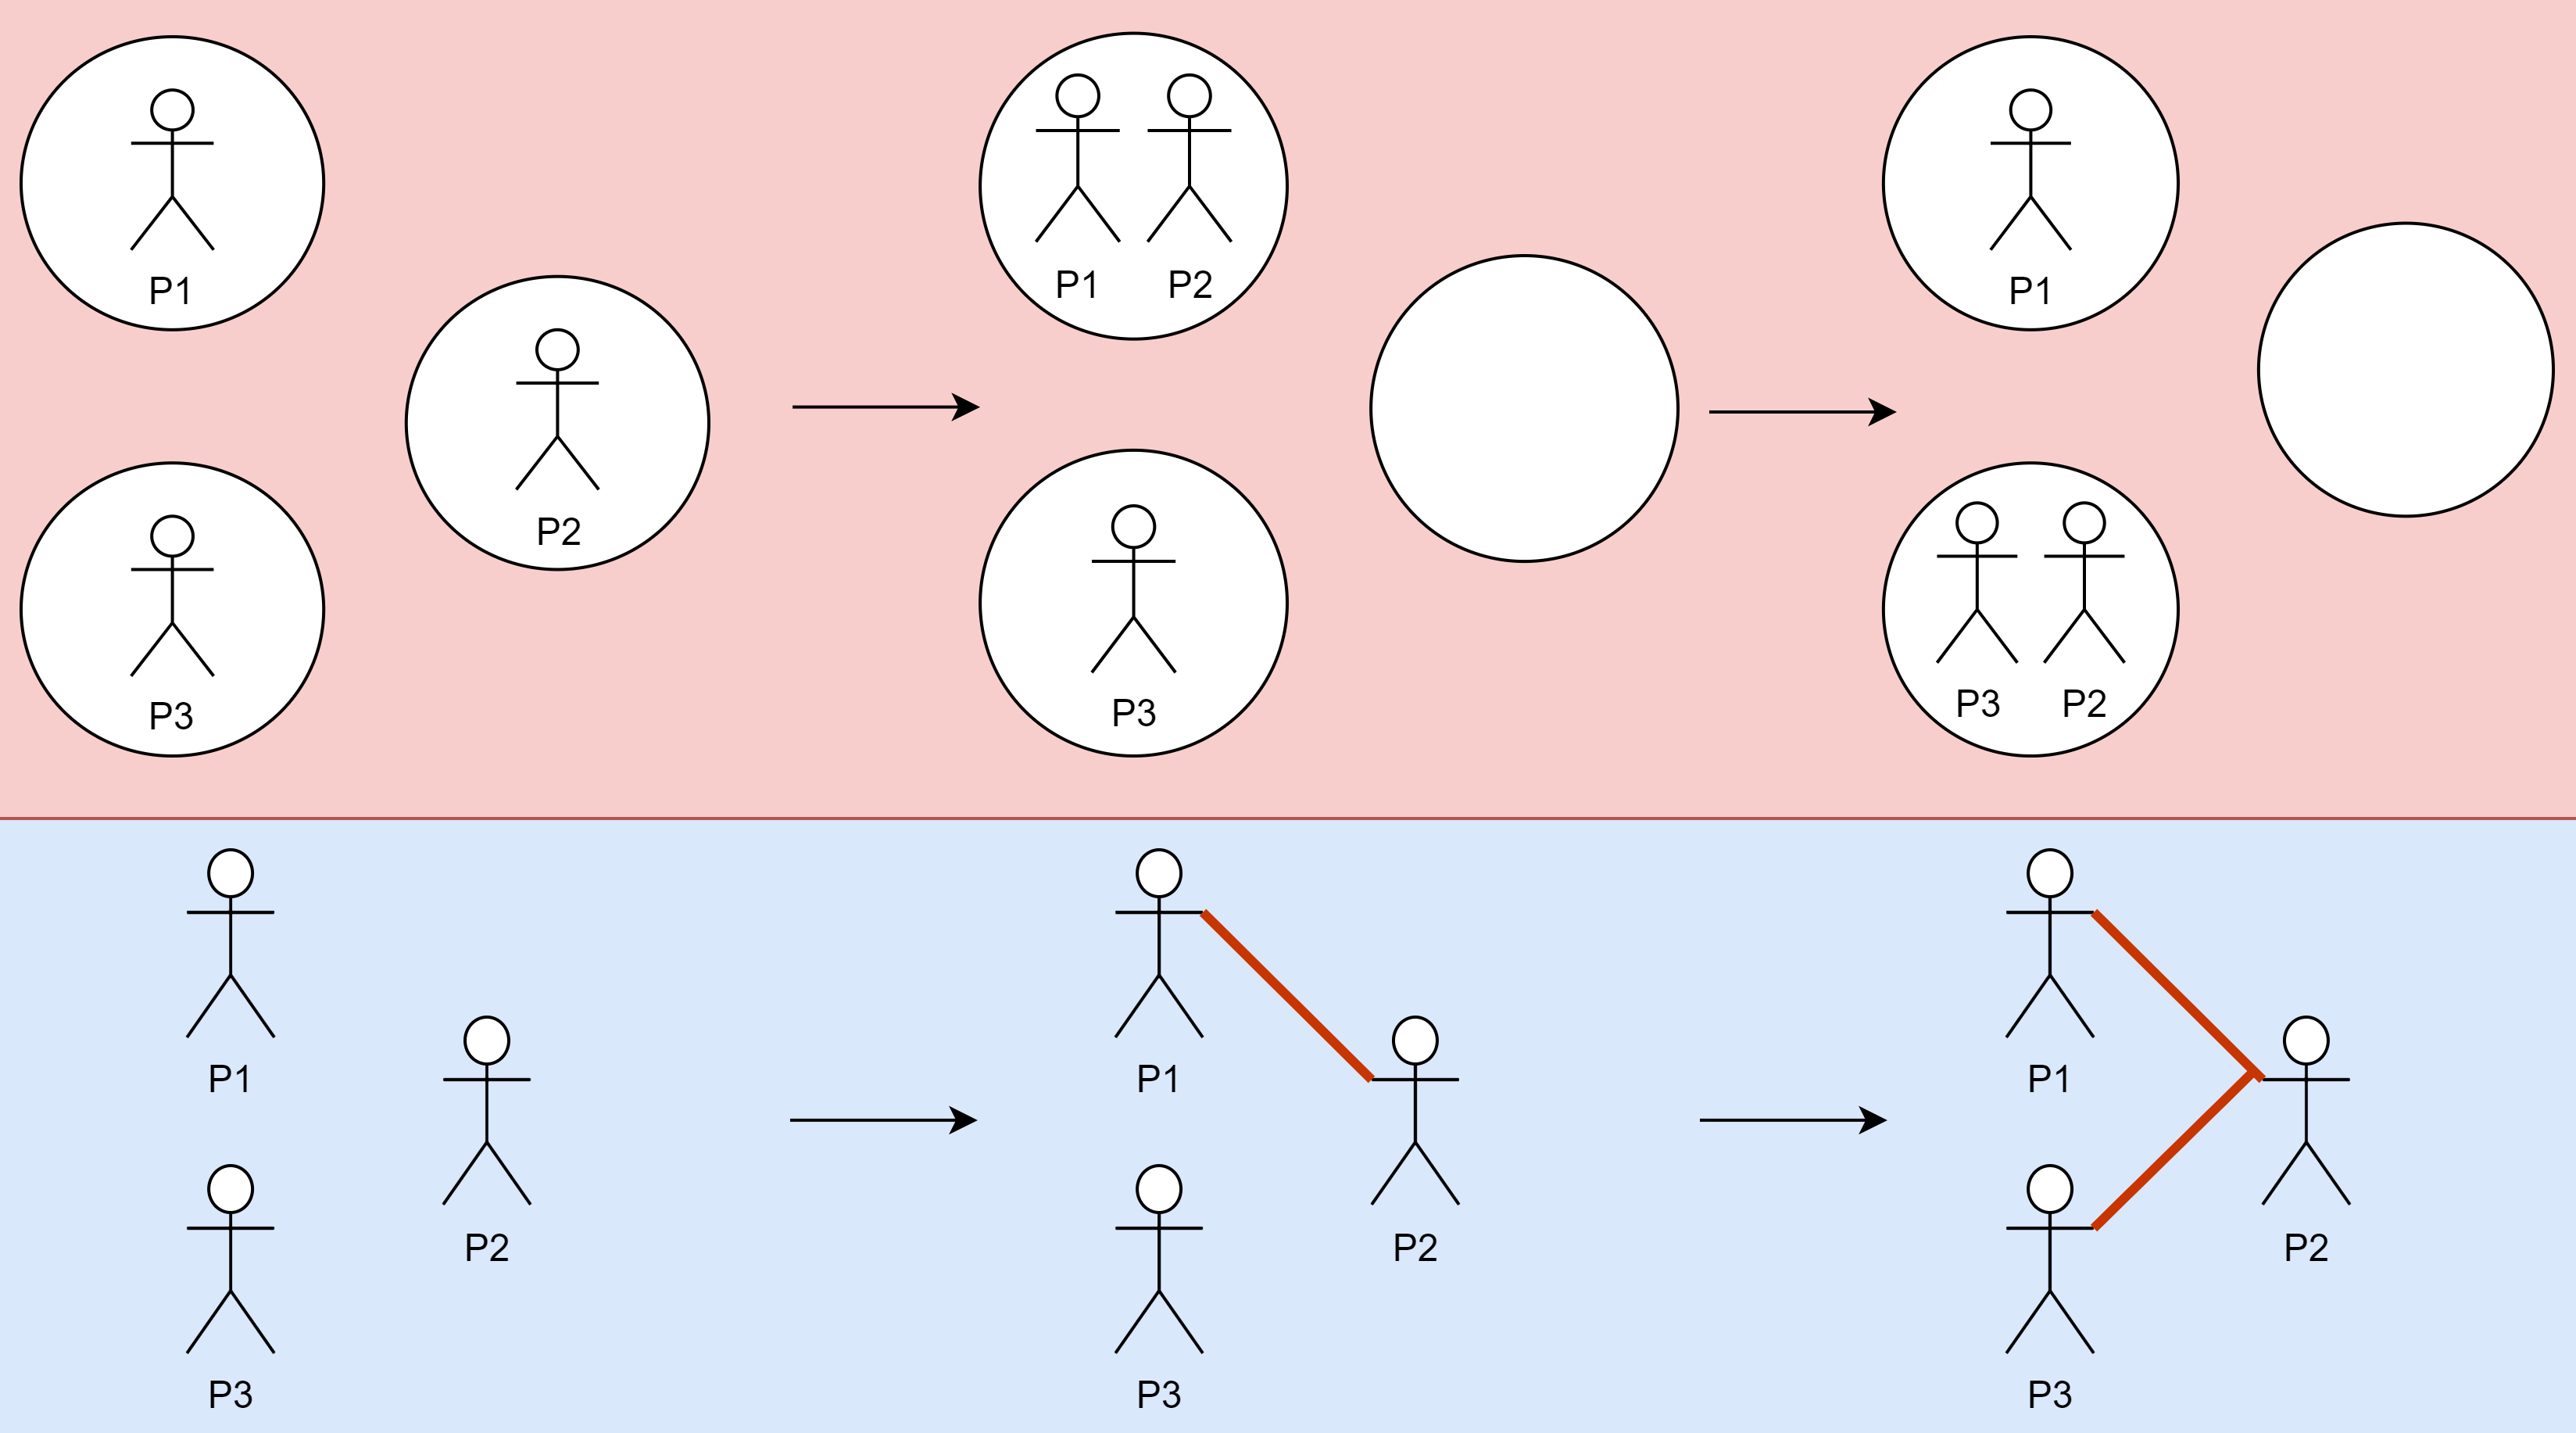
\includegraphics[width=0.30\textwidth]{imgs/Network_Toy.png}
    \caption{Example of contact network generation}
    \label{fig:toy_label}
\end{figure}

Then we also created a set of 62 contact networks, one for each day from July 1st, 2020 to August 31st, 2020. We used the same logic as before to create these individual contact networks. If two people were at the same location at the same time for at least 60 minutes, we created an edge between them. We will call this set of networks the Temporal Contact Networks. Each day's network captures the meaningful contacts that occurred between people for that day. Furthermore, we analyzed how the clustering coefficient and average node degree changed over time by calculating these metrics for each network in the Temporal Contact Networks.

Furthermore, we created an SIR simulation using the Temporal Contact Networks, which we ran from July 1st, 2020 to August 31st, 2020. Here are the parameters and assumptions that were made for the simulation:
\begin{itemize}[itemsep=0pt]
    \item Contact between people that is less than 60 minutes is not considered significant enough to spread the virus.
    \item If a susceptible person comes into contact with an infected person for at least one hour, then they get infected with a probability of 0.30. This is called the infection rate (IR) and it is constant.
    \item An infected person will recover after seven days. This is called the recovery period (RP) and it is constant.
    \item A person can only be infected if they were previously susceptible, and a person can only be recovered if they were previously infected.
    \item Initially, 20\% of the people, chosen at random, are infected. The rest are susceptible.
    \item Only infected people can infect others.
\end{itemize}

The simulation algorithm is shown in Algorithm \ref{alg:sir}. The simulation was run on each network in the Temporal Contact Networks. The simulation results were analyzed to see how the virus spread over time. This approach is scaleable, as the simulation can be run on any number of Temporal Contact Networks. Thus, we can use this approach to simulate the spread of the virus over a longer period of time.

\begin{algorithm}
\caption{SIR Simulation}
\label{alg:sir}
\begin{minipage}{\linewidth}
\scriptsize
\begin{algorithmic}
    \STATE \textbf{Input:} Temporal Contact Networks (TCN: Array of Contact Networks), IR, RP
    \STATE \textbf{Initialize:} Set 20\% nodes with $state$ = $I$, Set 80\% nodes with $state$ = $S$, Set all nodes with $time\_of\_recovery$ = $\infty$
\FOR {$i$ = 1 to len(TCN)}
    \FOR {each node $n$ where $n.state$ = $I$}
        \FOR {each neighbor $m$ of $n$ in TCN$[i]$ where $m.state$ = $S$}
            \IF {$rand(0, 1)$ $<=$ IR}
                \STATE $m.state$ = $I$
                \STATE $m.time\_of\_recovery$ = $i + RP$
            \ENDIF
        \ENDFOR
        \IF {$i$ = $n.time\_of\_recovery$}
            \STATE $n.state$ = $R$
        \ENDIF
    \ENDFOR
\ENDFOR
\end{algorithmic}
\end{minipage}
\end{algorithm}

\subsection{Machine Learning}

% there was an overlap of at least 60 minutes in their dwelling times, we considered this as a contact between the two people. We then added an edge between the two people in our graph.

% Separately, we also created a sample Susceptible-Infected (SI) simulation using data from July 1st, 2020. We did not include a recovery/death or incubation period in this model mainly because we only performed the simulation over one day. For the simulation, we did the following: at hour 0, we randomly infected 20\% of the nodes in the graph. Then we looked at all contacts between people for hour 1, and if an infected person came into contact with a susceptible person, we created an edge between them and infected the susceptible person with a probability of 1. We repeated the previous step for the remaining 22 hours of the day.

After generating and analyzing the 5-Day Contact Network, and Temporal Contact Networks, and performing the SIR simulation, we moved towards leveraging graph learning techniques to perform link prediction, which is the fundamental task behind automating contact tracing. Initially, we focused on performing link prediction on a static graph. In order to have enough data to train and evaluate our models, we used the 5-Day Contact Network. 

\subsubsection{Static Link Prediction}
Our first goal was to create a baseline link prediction model. We used the node2vec algorithm to generate node embeddings for each node in the graph \cite{grover2016node2vec}. We then generated the dataset of edges. To perform link prediction, we need a set of positive edges, which are the edges present in the network, and we need a set of negative edges, which are the edges not present in the network. This allows us to boil down the link prediction to a binary classification problem. Given our network, we created a set of negative edges that was equal in size to the set of positive edges to ensure balanced training. Using the node2vec embeddings and the set of positive and negative edges, we trained a GraphSAGE model to perform link prediction on the static 5-Day Contact Network \cite{hamilton2018inductive}.

\begin{figure}
    \centering
    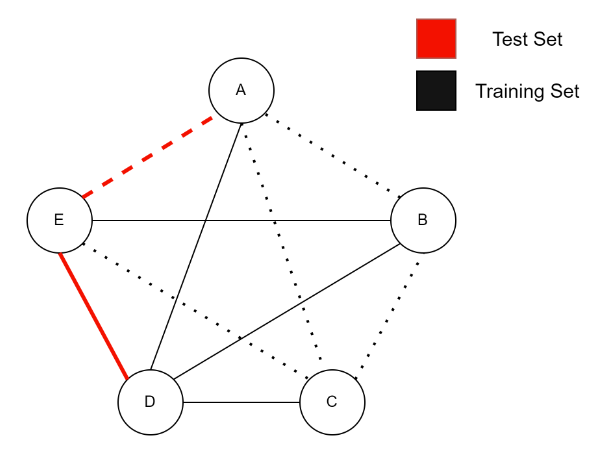
\includegraphics[width=0.25\textwidth]{imgs/static_prediction_data_split.png}
    \caption{Example of positive and negative edges for train and test data}
    \label{fig:toy_edges_label}
\end{figure}

A sample example of training and testing data is shown in Figure \ref{fig:toy_edges_label}. The black lines represent training data and the red lines represent testing data. The solid lines represent positive edges and dotted lines represent negative edges. The model is trained on the black lines, and attempts to predict the red lines. This allows us to boil down the link prediction to a binary classification problem.

After creating the baseline model, we searched for ways to improve the model's performance on the graph. This would include performing feature engineering techniques to add dimensions to our node embeddings and exploring the use of other GNN architectures such as the Graph Convolutional Network (GCN) and/or the Graph Attention Network (GAT) \cite{kipf2017semisupervised} \cite{veličković2018graph}. We hoped to be able to finetune the model and improve its performance to the point we could use it to perform link prediction on the Temporal Contact Networks. This approach is scalable because generating the training and testing edge sample, node embeddings, and node features can be done on a network of any size; however, generating the node2vec embeddings for a large network can be computationally expensive.

\subsubsection{Temporal Link Prediction}
After performing static link prediction on the 5-Day Contact Network, we moved towards performing temporal link prediction on the Temporal Contact Networks. 


\Section{Experimental Setup and Results}

% \begin{figure}
%     \centering
%     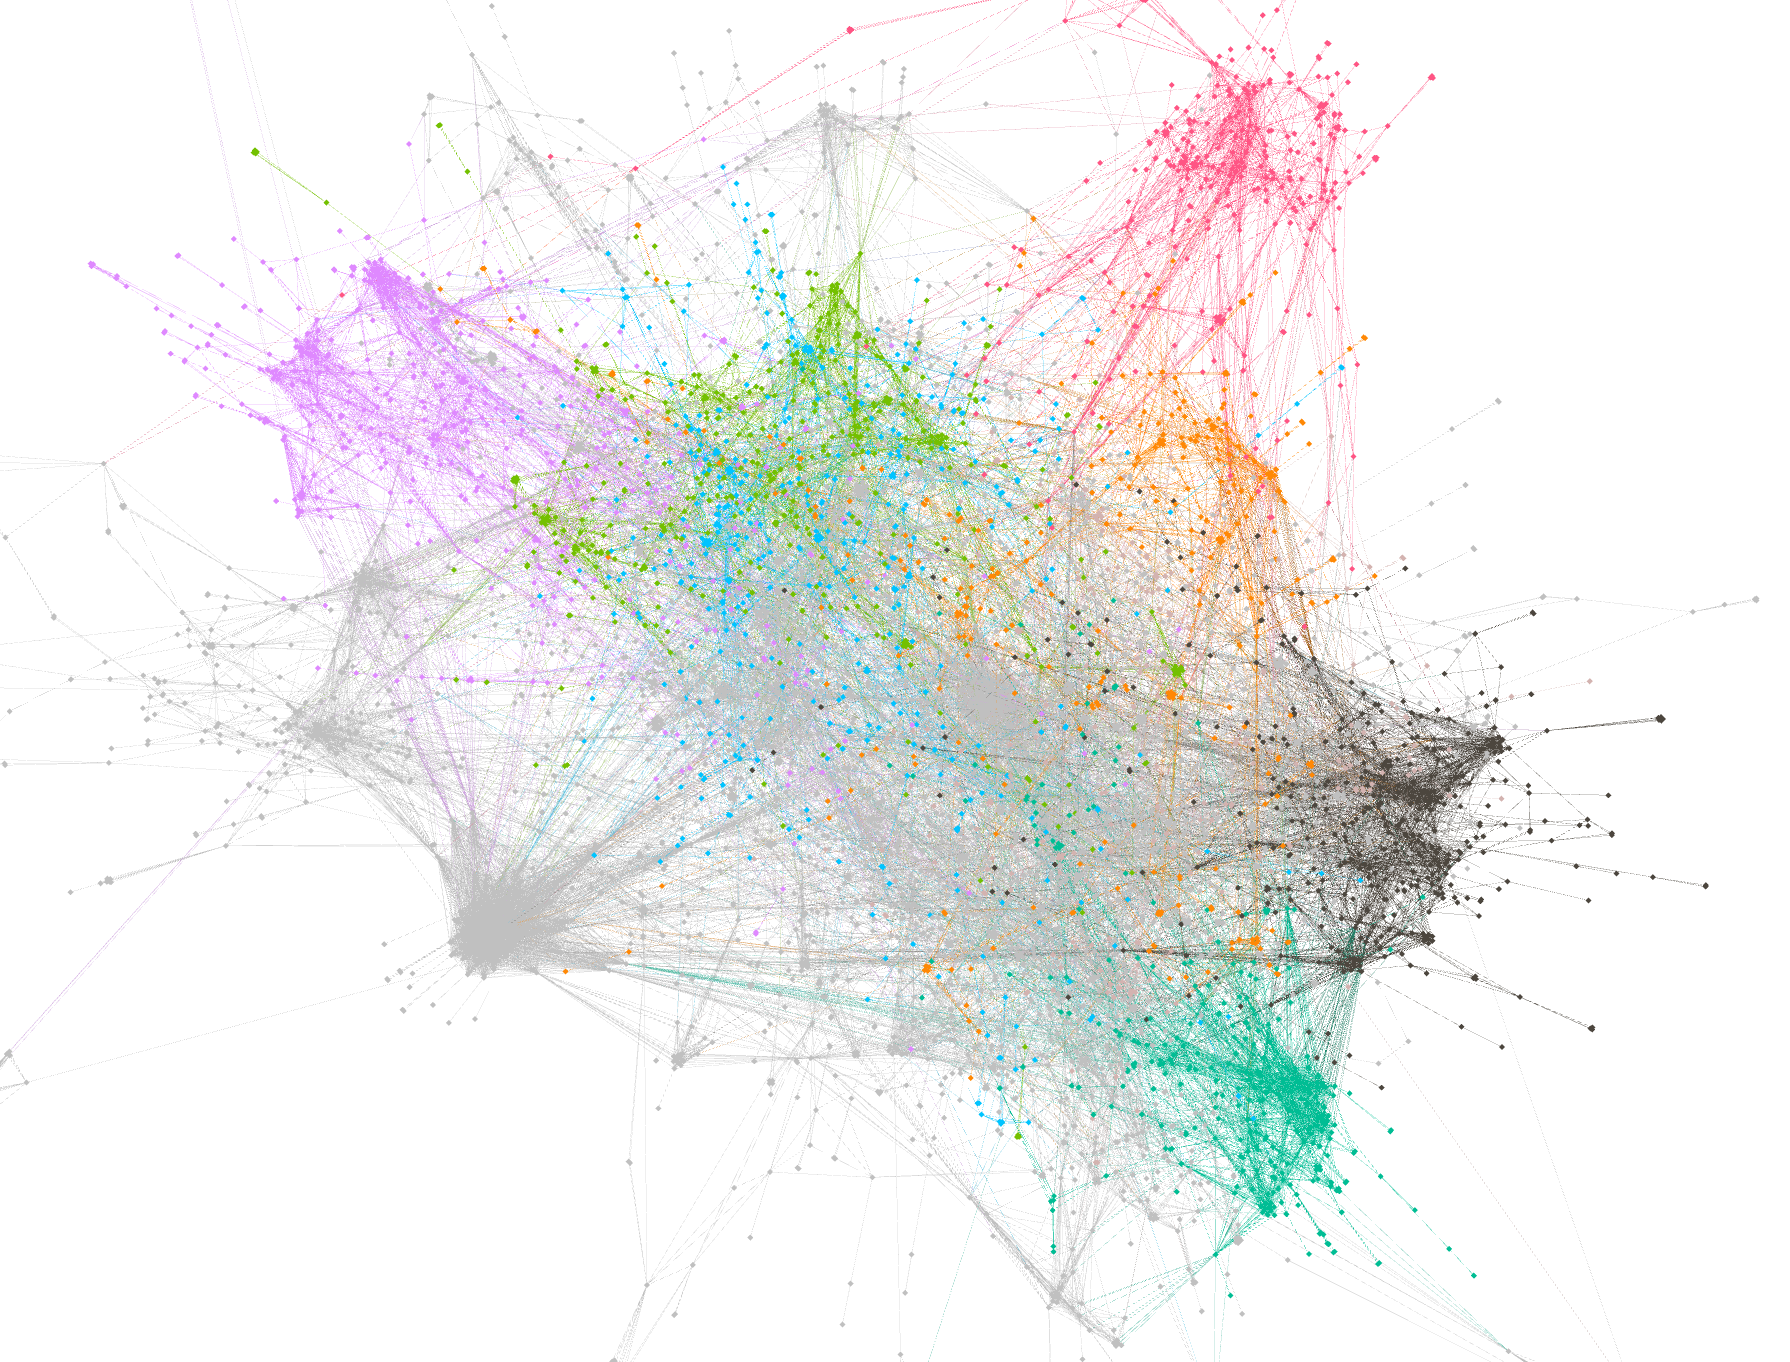
\includegraphics[width=0.23\textwidth]{imgs/one_day_net.png}
%     \caption{Contact network after one day}
%     \label{fig:my_label}
% \end{figure}

\vspace{-15pt}
\begin{figure}[h]
    \centering
    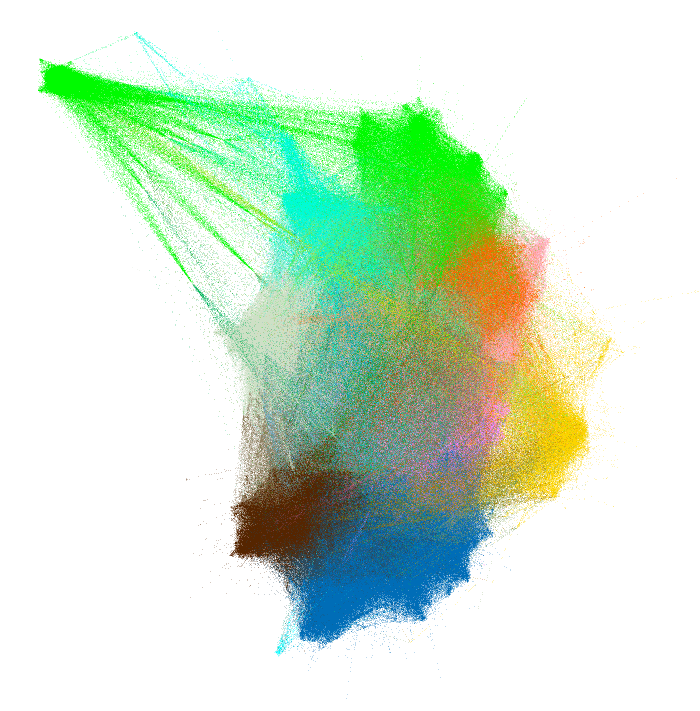
\includegraphics[width=0.15\textwidth]{imgs/5_day_network.png}
    \caption{5-Day Contact Network from July 1st, 2020 to July 5th, 2020}
    \label{fig:my_label}
\end{figure}

\vspace{-15pt}
\begin{figure}[h]
    \centering
    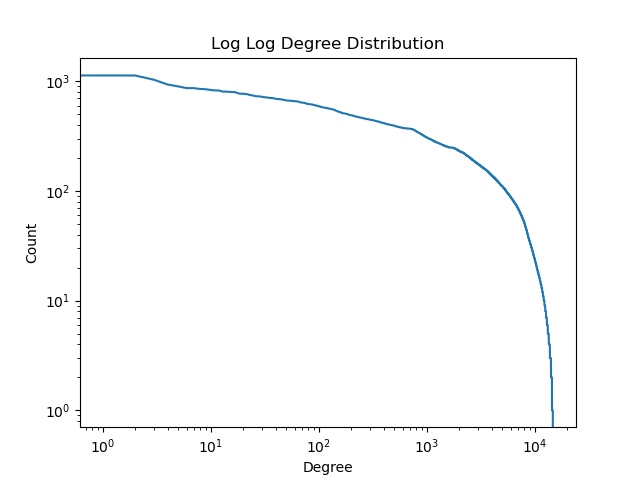
\includegraphics[width=0.23\textwidth]{imgs/5_day_log_log_degree_distribution.png}
    \caption{5-Day Contact Network Degree Distribution}
    \label{fig:deg_dist}
\end{figure}

In Figure \ref{fig:my_label}, we can see the 5-Day Contact Network. Network properties for this network were calculated. The average node degree is 102.599, the network diameter is 7, the average clustering coefficient is 0.627, and the average path length is 2.849. In addition to this, the degree distribution was mainly an exponential distribution with subtle hints of power-law as shown in Figure \ref{fig:deg_dist}. This can be seen from the network itself, as we can see the presence of a few hubs in the network.

% This can also be seen from the network itself, as we can see the presence of a few hubs in the network. This makes sense, as we should expect a social network to be scale-free, but we do not have all the data points, so it is not fully scale-free on the .


\begin{figure}[h]
    \centering
    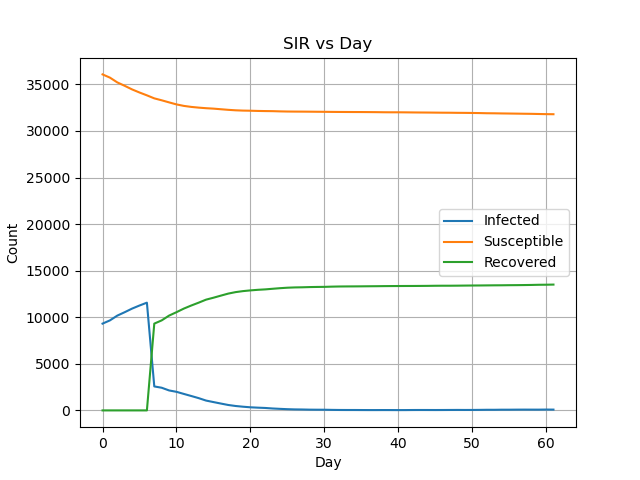
\includegraphics[width=0.30\textwidth]{imgs/complete_simulation.png}
    \caption{SIR Simulation Results}
    \label{fig:simulation_results}
\end{figure}

In addition, the simulation results are shown in Figure \ref{fig:simulation_results}. The simulation results show that the number of infected people initially increases, but then decreases significantly and approaches zero. However, the number of recovered people exhibits the opposite behavior. This makes sense since the people who started with the infection at the beginning of the simulation recover after seven days; thus, they can no longer infect others nor become susceptible again. Also, the number of susceptible people decreases over time, which makes sense since they are getting infected and recovering. The maximum number of infected people on any given day is about 11,500 and the total number of people infected over the simulation is about 14,300.

It is important to note that this simulation was run on limited data. The total number of nodes in the simulation, which is the total number of people, is around 45,000, whereas the actual population in the Austin metropolitan area in 2020 was around 2 million. Furthermore, this model assumes a closed population, which is not the case in Austin, TX. People are constantly moving in and out of the city. Thus, the simulation results are not representative of the actual spread of the virus in Austin, TX.  Having access to more data would allow the simulation to provide realistic results. However, this simulation does show that the virus can spread quickly, as seen in the first week of the simulation. Thus, it is important to have an efficient and accurate contact tracing system to mitigate the spread of the virus.

\begin{figure}[h]
    \centering
    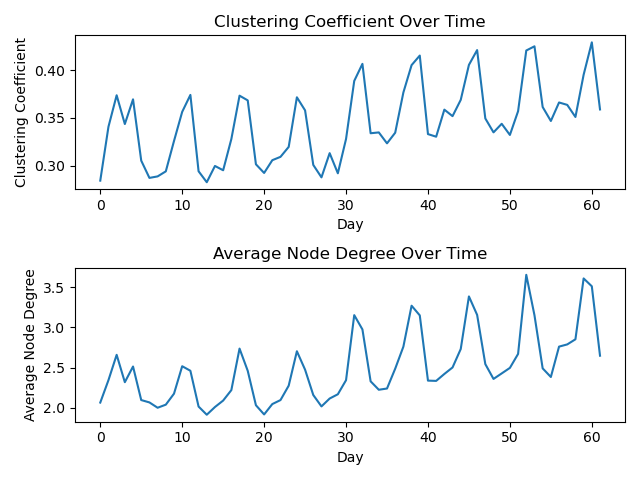
\includegraphics[width=0.3\textwidth]{imgs/temporal_network_analysis.png}
    \caption{Clustering Coefficient and Average Node Degree for Temporal Contact Networks} 
    \label{fig:temporal_stats}
\end{figure}

We also analyzed the Temporal Contact Networks. The clustering coefficient and the average node degree for these networks are shown in Figure \ref{fig:temporal_stats}. The results reveal a seven-day periodic pattern with peaks occurring on the weekends. These results make sense since people are more likely to go out and socialize on the weekends. This increase in socialization on the weekends leads to more contacts, which leads to a higher clustering coefficient and average node degree.

After performing the analysis on the 5-Day Contact Network and Temporal Contact Networks, we moved towards performing link prediction on the 5-Day Contact Network. For our baseline model, as stated in the approach, we used a GraphSAGE model with node2vec embeddings. We trained the model for 1000 epochs on a 90/10 train/test split with the Adam optimizer \cite{kingma2017adam}. The model achieved an AUC score of 0.49 on the test data, which is worse than random guessing. Part of this could be because no internal node features were used in the node embeddings.

To improve upon this, we performed feature engineering to generate additional features for each node. The features we added included average number of locations traveled to per day, average distance traveled per day, age, gender, and State-Age-Gender (SAG) score. By adding these features to the node2vec embeddings, we were able to improve the AUC score to 0.63, which is a significant improvement over the baseline model. We can see that the additional features helped the model learn the graph structure better. 

% We then attempted to improve upon this by taking the features we generated and normalizing them before appending them. We saw that the features were all of different scales compared to each other and the node2vec embeddings, so we hypothesized that normalizing the features would improve the model's performance. This, again, improved our model's performance, as we were able to achieve an AUC score of 0.75.

We noticed that the features were of different scales, so we hypothesized that normalizing the features would improve the model's accuracy. This adjustment improved the performance of the model, leading to an AUC of 0.75.

Seeking further enhancement, we explored a different model architecture, specifically the GCN model. Utilizing the same features and data, the GCN model achieved an AUC score of 0.91, demonstrating a significant improvement over the initial model.

% From these performance metrics, we can see that performing link prediction on the Temporal Contact Networks is a feasible task. We can also see that the GCN model performs significantly better than the GraphSAGE model. Thus, we plan to use the GCN model to perform link prediction on the Temporal Contact Networks for M3.

While these performance metrics establish the feasibility of link prediction on contact networks, it's crucial to note a limitation in the current approach—namely, its inability to capture temporal data. Recognizing this limitation, our next objective for M3 is to implement temporal link prediction using the GCN model. This aligns with our goal of automating contact tracing.

% In addition, we can see the resulting infected graph from our simulation in Figure \ref{fig:my_label2}.
% \begin{figure}
%     \centering
%     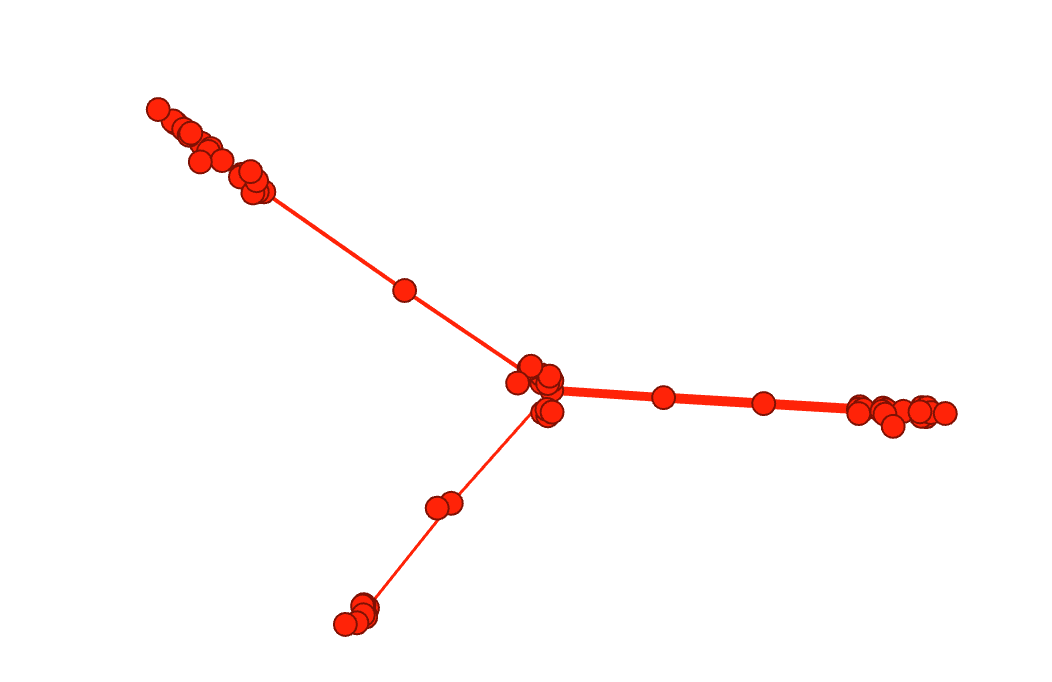
\includegraphics[width=0.23\textwidth]{imgs/simulation.png}
%     \caption{Infected graph after one day}
%     \label{fig:my_label2}
% \end{figure}
% In this network, it is important to note that all of the visible nodes are infected, and the edges represent how the infection has been spread. We can see that not a lot of infected nodes have spread the virus, but the ones that have created one connected component that show the beginnings of a scale-free network. 

% In Figure \ref{fig:my_label3}, we can see the number of infected nodes over time. We can see that the infection doesn't spread much until the latter half of the day, after which it spreads steadily. We expect the rate of spread to be exponential when we simulate the spread over more days. This lines up with our intuition, as we would expect the infection to spread faster as more people get infected.
% \begin{figure}
%     \centering
%     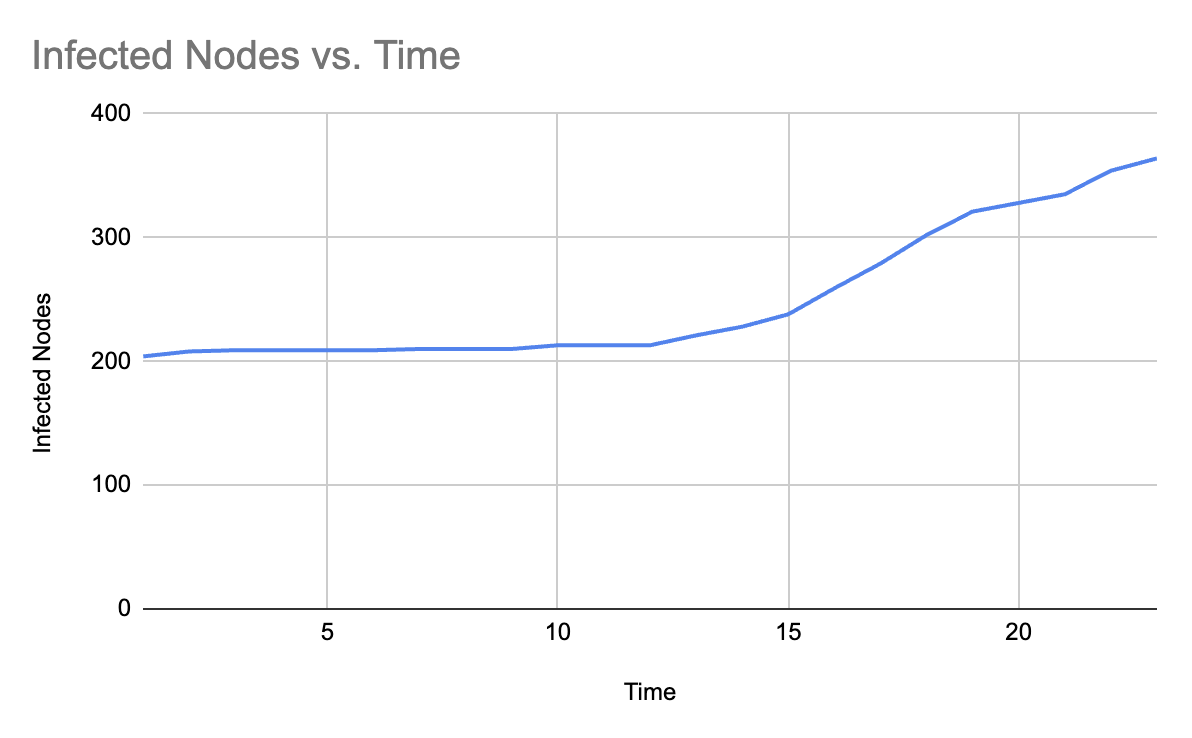
\includegraphics[width=0.28\textwidth]{imgs/infected_over_time.png}
%     \caption{Number of infected nodes over 24 hours}
%     \label{fig:my_label3}
% \end{figure}


\Section{Conclusion and Short-Term Plans}
Through the analysis of the 5-Day Contact Network, we were able to determine that the network is mostly exponential in degree distribution, with hints of scale-free properties. Some people came into contact with many other people whereas others stayed within their cliques. The simulation showed that the number of infected people initially increases, but after a few days, decreases significantly.

The analysis of the Temporal Contact Networks highlights a pattern in mobility. Particularly, people tend to socialize more on the weekends, which leads to a higher clustering coefficient and average node degree.

Finally, we were able to perform static link prediction on the 5-Day Contact Network. We were able to improve the model's performance by performing feature engineering and using the GCN model. 

For M3, we plan to use the Temporal Contact Networks for temporal link prediction. Essentially, given contact networks for July 1st, 2020 to August 15th, 2020, the model will attempt to predict the contacts that will occur from August 16th, 2020 to August 31st, 2020. We will also attempt to improve the model's performance by performing feature engineering and using other GNN architectures.

For this milestone, Afnan generated and analyzed the 5-Day Contact Network and performed static link prediction on it. Jaykumar created and analyzed the Temporal Contact Networks and ran the SIR simulation on them.


% For M2, we plan to do a more complete analysis of the network by considering both July and August data. We also plan to run more realistic simulations by accounting for the incubation period, deceased people, and recovered people. We also plan to implement GNNs at a small scale to perform link prediction. Specifically, we will use GNNs to predict the people that come into contact with previously infected people. By predicting contact between people, we will be able to predict the spread of the virus.

%------------------------------------------------------------------------- 
% \Section{Objectives and Deliverables}

% First, we will analyze the networks to determine their properties. Then, to better understand network behavior, we will run simulation to see how COVID-19 spreads through the network.

% The main goal of contact tracing is to find people who may be infected due to their contact with other infected people. Similarly, this project will aim to classify infected nodes in a graph, where nodes represent people, and links represent contact between people. This network will be formed by utilizing real contact information from mobile devices. In order to predict infections within a network, this project will implement and analyze GNNs, specifically link prediction. 

% The dataset we will be using is the ``foursquare'' mobility dataset that consists of location visit logs in Austin, TX from 2019 to 2021. The visit log includes information about when and where a device was, as well as how long it was there. 
% - What are the main research questions you plan to address?
% - How exactly is the “network” formed? What is a “node” and what is a “link”?
% - Which dataset(s) do you plan to use?
% - What are the deliverables?

%------------------------------------------------------------------------- 
% \Section{Tasks and Timeline}

% Firstly, we will collect and clean the data. This includes reformatting and filtering the data. We will analyze the dataset to get a better understanding of its properties (such as degree, betweenness centrality, clustering coefficient, etc.). We plan to complete this by October 10th, 2023.

% Then we plan to run simulations on the network to get a better understand of how the virus flows. We plan to complete this by November 14th, 2023.

% Finally, we will utilize GNNs to perform link prediction to see how the network evolves over time. We plan to complete this by November 30th, 2023.

% We will pair program; thus, the member contribution will be 50/50.

% - What are the main tasks of your project?
% - What is the proposed timeline (w.r.t. project milestones) and member(s) contribution?

%------------------------------------------------------------------------- 

% \Section{Conclusion and References}

% In conclusion, the project aims to utilize GNNs to make contact tracing more efficient and accurate. We will analyze the dataset to understand its properties, we will run simulations to see how the virus spreads through the network, and we will train GNNs to perform link prediction.

% We will start by researching GNNs. Particularly, we will look at an article by Neptune.ai on the application of GNNs and a DGL tutorial on link prediction \cite{menzli-blog} \cite{dglLinkPrediction}.

% https://towardsdatascience.com/graph-convolutional-networks-introduction-to-gnns-24b3f60d6c95
% https://neptune.ai/blog/graph-neural-network-and-some-of-gnn-applications#:~:text=Graph%20Neural%20Networks%20(GNNs)%20are,and%20graph%2Dlevel%20prediction%20tasks.
% https://docs.dgl.ai/en/0.8.x/tutorials/blitz/4_link_predict.html

% what a GNNs is, and how to use it (blogs on this).

% - Briefly summarize the project idea and main contributions.
% - Include some starting points (e.g., papers, websites, datasets, etc., preferably more than what
% was given to you as a starting point in the projects description).


%------------------------------------------------------------------------- 
% \nocite{ex1,ex2}
\bibliographystyle{latex8}
\bibliography{latex8}

\end{document}

